% Topic 32 — IterCOMP: Reasoning-aware Adaptive Prompt Compression
% ACL short paper. Than bai (§1 Intro .. §10 Conclusion) ~4.5 trang; References
% tu trang 5; phu luc sau do. Kiem layout: python scripts/check_layout.py
%
% Build:  pdflatex report && bibtex report && pdflatex report && pdflatex report
% acl.sty and acl_natbib.bst from https://github.com/acl-org/acl-style-files

\documentclass[11pt]{article}
\usepackage[final]{acl}

\usepackage{times}
\usepackage{latexsym}
\usepackage[T1,T5]{fontenc}   % T5 for Vietnamese examples
\usepackage[utf8]{inputenc}
\usepackage{microtype}
\usepackage{balance}
\usepackage{graphicx}
\usepackage{booktabs}
\usepackage{amsmath}
\usepackage{multirow}
\usepackage{tikz}
\usetikzlibrary{arrows.meta,positioning,calc,shapes.geometric,fit,backgrounds,decorations.pathreplacing,shadows,shapes.callouts}
\usepackage{xcolor}
% Bảng màu dịu, phân biệt được cả khi in đen trắng (độ sáng khác nhau rõ).
\definecolor{cData}{HTML}{E8EEF7}   % dữ liệu vào/ra  — xanh nhạt
\definecolor{cDataL}{HTML}{4A6FA5}
\definecolor{cScore}{HTML}{FDF0E3}  % khâu chấm điểm  — cam nhạt
\definecolor{cScoreL}{HTML}{C97B24}
\definecolor{cLLM}{HTML}{EAF3EA}    % khâu gọi LLM    — lục nhạt
\definecolor{cLLML}{HTML}{4E8A52}
\definecolor{cLoop}{HTML}{9B4D8C}   % vòng phản hồi   — tím

\title{When Compression Meets Diacritics: IterCOMP-VN for\\
Vietnamese Multi-hop Question Answering}

\author{
  \begin{tabular}{ccc}
    Trương Thành Nhân & Trần Ngọc Vỹ & Trần Nhật Minh \\
  \end{tabular} \\[0.4em]
  Faculty of Information Technology, VNUHCM - University of Science, Ho Chi Minh City, Vietnam \\
  \texttt{\{25C1505320, 25C1506947, 24C11055\}@student.hcmus.edu.vn}
}

\begin{document}
\maketitle

\begin{abstract}
Multi-hop question answering burdens retrieval-augmented generation with long,
noisy contexts, and prompt compression is a natural remedy. IterCOMP
\citep{yun2026itercomp}, a state-of-the-art training-free compressor, reports
strong results but is evaluated only on English. We reimplement it and give it,
to our knowledge, its first systematic evaluation on Vietnamese, using the
complete VimQA benchmark \citep{le2022vimqa}. Sentence-level compression reliably
beats token-level alternatives, yet the fuller method ordering is
reader-dependent: a stronger reader tolerates distractor noise and gains more
from uncompressed context, so compression's accuracy advantage is not intrinsic.
Vietnamese also surfaces effects English hides: tokeniser fertility makes nominal
compression ratios understate the real token cost by $2.39\times$, which we
correct with an \emph{effective ratio}; a boolean-answer normalisation step is
worth $+10.0$ F1 in Vietnamese but nothing in English; and on undiacriticised
text - ubiquitous online - compressed context can outscore even gold context.
We release our implementation and Vietnamese prompts to support reproducibility.
\end{abstract}

\section{Introduction}
\label{sec:intro}

Multi-hop question answering requires aggregating evidence across documents.
Retrieval-augmented generation (RAG) \citep{lewis2020rag} supplies external
documents to compensate for a model's bounded knowledge, but introduces two
problems: \emph{cost} (input length grows linearly with the number of documents)
and \emph{noise} (irrelevant passages degrade reader accuracy).

\begin{figure*}[t]
\centering
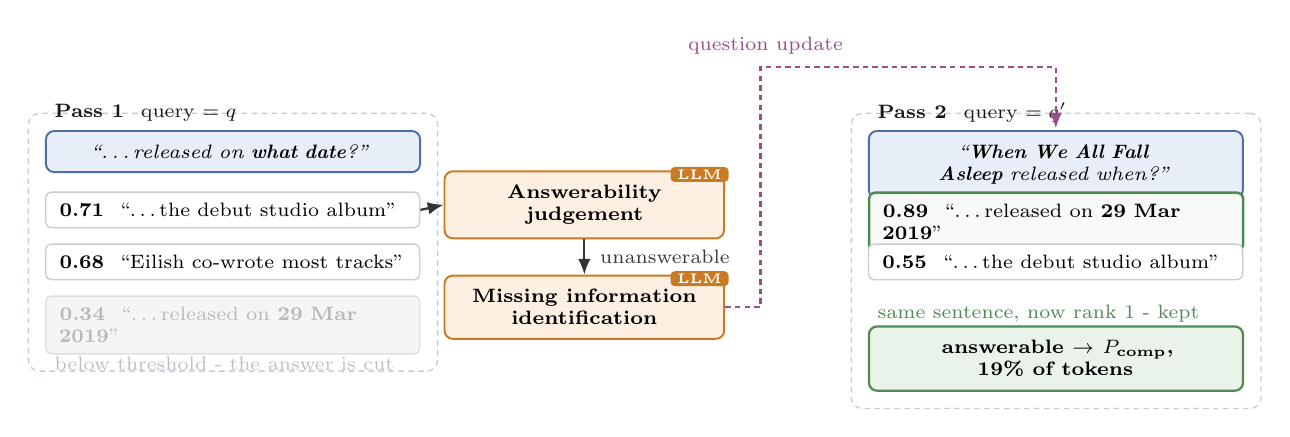
\begin{tikzpicture}[
  font=\footnotesize, x=1cm, y=1cm,
  % ── mot bang mau duy nhat: xanh = du lieu, cam = LLM, luc = ket qua ──
  qq/.style={rounded corners=3pt, draw=cDataL, fill=cData, line width=0.7pt,
             align=center, font=\scriptsize, text width=44mm,
             inner xsep=5pt, inner ysep=5pt},
  sg/.style={rounded corners=2pt, draw=gray!40, fill=white, line width=0.5pt,
             align=left, font=\scriptsize, text width=44mm,
             inner xsep=5pt, inner ysep=4pt},
  kp/.style={sg, draw=cLLML, fill=cLLM!40, line width=0.9pt},
  dp/.style={sg, draw=gray!25, fill=gray!8, text=gray!55},
  ai/.style={rounded corners=3pt, draw=cScoreL, fill=cScore, line width=0.7pt,
             align=center, font=\scriptsize\bfseries, text width=32mm,
             inner xsep=5pt, inner ysep=5pt},
  ok/.style={rounded corners=3pt, draw=cLLML, fill=cLLM, line width=0.8pt,
             align=center, font=\scriptsize\bfseries, text width=44mm,
             inner xsep=5pt, inner ysep=5pt},
  tag/.style={font=\tiny\bfseries, text=white, fill=cScoreL, rounded corners=1.5pt,
              inner xsep=2.5pt, inner ysep=1pt},
  a/.style={-{Latex[length=2mm,width=1.6mm]}, line width=0.8pt, gray!40!black},
  b/.style={-{Latex[length=2mm,width=1.6mm]}, line width=0.9pt, cLoop,
            dashed, dash pattern=on 2pt off 1.5pt},
  hd/.style={font=\scriptsize\bfseries, text=gray!20!black, anchor=west},
  nt/.style={font=\scriptsize, align=left, anchor=north west},
]
% ═══ luoi: cot x = 0 / 6.4 / 10.6 ; hang y cach deu 0.72 ═══
\def\cL{0}      \def\cM{6.85}   \def\cR{10.45}

% ── PASS 1 ───────────────────────────────────────────────
\node[hd] at (\cL,2.72) {Pass 1 \ \textnormal{query $=q$}};
\node[qq, anchor=north west] (q1) at (\cL,2.50)
  {\emph{``\dots released on \textbf{what date}?''}};
\node[sg, anchor=north west] (s1) at (\cL,1.72)
  {\textbf{0.71} \ ``\dots the debut studio album''};
\node[sg, anchor=north west] (s2) at (\cL,1.06)
  {\textbf{0.68} \ ``Eilish co-wrote most tracks''};
\node[dp, anchor=north west] (s3) at (\cL,0.40)
  {\textbf{0.34} \ ``\dots released on \textbf{29 Mar 2019}''};
\node[nt, text=gray!50] at (\cL,-0.26)
  {below threshold - the answer is cut};

% ── LLM ──────────────────────────────────────────────────
\node[ai] (j1) at (\cM,1.55) {Answerability\\ judgement};
\node[tag, anchor=north east] at ($(j1.north east)+(0.05,0.05)$) {LLM};
\node[ai] (j2) at (\cM,0.25) {Missing information\\ identification};
\node[tag, anchor=north east] at ($(j2.north east)+(0.05,0.05)$) {LLM};
\draw[a] (s1.east) -- (j1.west);
\draw[a] (j1) -- node[font=\scriptsize, right=2pt, text=gray!45!black]
         {unanswerable} (j2);

% ── PASS 2 ───────────────────────────────────────────────
\node[hd] at (\cR,2.72) {Pass 2 \ \textnormal{query $=q'$}};
\node[qq, anchor=north west] (q2) at (\cR,2.50)
  {\emph{``\textbf{When We All Fall Asleep} released when?''}};
\node[kp, anchor=north west] (t1) at (\cR,1.72)
  {\textbf{0.89} \ ``\dots released on \textbf{29 Mar 2019}''};
\node[sg, anchor=north west] (t2) at (\cR,1.06)
  {\textbf{0.55} \ ``\dots the debut studio album''};
\node[nt, text=cLLML] at (\cR,0.40) {same sentence, now rank 1 - kept};
\node[ok, anchor=north west] (rd) at (\cR,0.02)
  {answerable $\rightarrow$ $P_\text{comp}$, 19\% of tokens};

% ── vong lap: di vong LEN TREN, khong cat qua hop nao ──
\draw[b] (j2.east) -- ++(0.45,0) |- (9.15,3.30) -| ($(q2.north)+(0,0.02)$);
\node[font=\scriptsize, text=cLoop, anchor=south] at (9.15,3.34)
  {question update};

\begin{scope}[on background layer]
  \node[fit=(q1)(s1)(s2)(s3), draw=cDataL!35, dashed, line width=0.5pt,
        dash pattern=on 2pt off 1.6pt, rounded corners=4pt, inner sep=6pt] {};
  \node[fit=(q2)(t1)(t2)(rd), draw=cLLML!35, dashed, line width=0.5pt,
        dash pattern=on 2pt off 1.6pt, rounded corners=4pt, inner sep=6pt] {};
\end{scope}
\end{tikzpicture}
\caption{One VimQA question through two IterCOMP passes. The sentence carrying the
release date scores $0.34$ and is filtered out, so a single-pass compressor loses
the answer; re-scored against the follow-up $q'$ it rises to $0.89$ and is kept.}
\label{fig:arch}
\end{figure*}

Prompt compression addresses both. However, existing methods
\citep{jiang2023llmlingua,pan2024llmlingua2,xu2024recomp,li2023selectivecontext}
compress \emph{once}, conditioned on the original question, and therefore miss the
defining property of multi-hop QA: the information needed at a later hop only
becomes identifiable after the evidence of the earlier hop is in hand.
IterCOMP \citep{yun2026itercomp} embeds multi-hop reasoning into the compression
loop itself. No public implementation accompanies the original paper, and its evaluation
remains restricted to English.

The Vietnamese adaptation and evaluation are our primary contribution; the
reproduction that enables them is reported subsequently. Our study contributes
five findings, four of them specific to Vietnamese:
(1)~a boolean-answer normalisation step worth $+10.0$ F1 on Vietnamese
($p=0.01$) and $0.0$ on English ($p=1.00$), a linguistic fix rather than a
metric-inflating one;
(2)~evidence that the iteration budget saturates beyond two passes, with
\texttt{max\_iter} from 2 to 5 moving F1 by $+1.2$ at $n=500$ (within noise)
while retention grows from 0.160 to 0.194;
(3)~an \emph{effective ratio} showing that nominal compression ratios understate
real token cost on Vietnamese by $2.39\times$, since the tokeniser that bills is
not the one that counts;
(4)~that Vietnamese does not handicap the compressor, IterCOMP reaching 84\% of
the Oracle ceiling on VimQA, the lower 54\% on English MuSiQue being a dataset
property, not a language effect (Appendix~\ref{app:decomp}); and
(5)~that on undiacriticised Vietnamese, compressed context beats gold context by
3.78 to 5.82 F1 (Appendix~\ref{app:undia}).
We call the resulting configuration IterCOMP-VN, and stress that it is \emph{not}
a new algorithm - the loop is unchanged; it is a deployment configuration plus a
metric-level fix, and we report below which parts survive significance testing.

None of this is measurable without a working reimplementation; absent a public
one, we rebuild it from the paper's description and redesign every prompt. It
recovers the central result on all four datasets (Table~\ref{tab:4ds});
Section~\ref{sec:vspaper} and Appendix~\ref{app:4ds} compare our numbers with the
original's dataset by dataset.

\section{Related Work}
\label{sec:related}

\paragraph{Prompt compression.} \emph{Extractive} methods retain a subset of tokens
or sentences: LLMLingua \citep{jiang2023llmlingua} uses perplexity from a small
model to drop uninformative tokens; LongLLMLingua
\citep{jiang2024longllmlingua} adds query awareness; LLMLingua-2
\citep{pan2024llmlingua2} recasts the task as token classification, which is far
faster and \emph{multilingual} - the decisive property for our Vietnamese
experiments; Selective-Context \citep{li2023selectivecontext} removes redundant
lexical units. \emph{Abstractive} methods regenerate shorter content, notably
RECOMP \citep{xu2024recomp}. All compress in a single pass.

\paragraph{Iterative retrieval.} Self-Ask \citep{press2023selfask} and IRCoT
\citep{trivedi2023ircot} decompose questions and interleave retrieval with
reasoning; IterCOMP instead \emph{narrows} the context rather than expanding it.

\paragraph{Vietnamese NLP.} Foundation models include PhoBERT
\citep{nguyen2020phobert} and ViT5 \citep{phan2022vit5}; to our knowledge, none
evaluates prompt compression for Vietnamese.

\section{Dataset}
\label{sec:dataset}

The three English datasets are standard for multi-hop QA and are exactly those
used by the original paper. VimQA \citep{le2022vimqa} is a Vietnamese
multi-hop QA dataset built from Vietnamese Wikipedia, annotated with reasoning
type (bridge / comparison) and gold supporting sentences; crucially,
it uses the same format as HotpotQA, so our code runs on Vietnamese
essentially unchanged. We use the distractor setting for all four, giving
10-20 candidate passages per question, so no Wikipedia index is required
and cost is per question rather than per corpus. Because MuSiQue
withholds test answers, we report on development sets throughout, and all four
datasets are evaluated under a single reader (Qwen2.5-7B at 4-bit) so the numbers
compare like with like; Table~\ref{tab:datasets} gives the statistics.

\begin{table}[t]
\centering
\small
\begin{tabular}{llrr}
\toprule
Dataset & Lang. & \#Q & \#psg \\
\midrule
HotpotQA (distractor) & En & 7,405  & 10 \\
2WikiMultiHopQA       & En & 12,576 & 10 \\
MuSiQue-Ans           & En & 2,417  & 20 \\
\textbf{VimQA}        & \textbf{Vi} & \textbf{1,003} & \textbf{10} \\
\bottomrule
\end{tabular}
\caption{Datasets (development-set statistics).}
\label{tab:datasets}
\end{table}

\section{Method}
\label{sec:method}


Given a question $q$ and document set $D$, we seek a compressed context
$P_{\text{comp}}$ with $|P_{\text{comp}}| \ll |D|$ such that the reader still
answers correctly. IterCOMP is training-free: all parameters stay frozen.
Each document is decomposed into sentence-level evidence segments $e_{i,j}$.
Figure~\ref{fig:arch} traces one question through two iterations.


\subsection{Relevant evidence filtering}
The \emph{semantic} signal is the inner product of dense representations from a
text encoder $E(\cdot)$:
\begin{equation}
S_{\text{sem}}(q, e_{i,j}) = E(q)^\top E(e_{i,j}).
\end{equation}
This can miss exact lexical cues. Following M3-Embedding
\citep{chen2024bgem3}, the importance weight of token $t$ is
\begin{equation}
w_t = \mathrm{ReLU}(\mathbf{w}_{\text{lex}}^\top E(t)),
\end{equation}
where $\mathbf{w}_{\text{lex}}$ is a projection vector. The \emph{lexical} score is a sparse
inner product over co-occurring tokens:
\begin{equation}
S_{\text{lex}}(q, e_{i,j}) = \sum_{t \in q \cap e_{i,j}} w_t^{q} \cdot w_t^{e_{i,j}}.
\end{equation}
The two are combined into a dual-aspect relevance score:
\begin{equation}
S_{\text{dual}} = \lambda \, S_{\text{sem}} + (1-\lambda) \, S_{\text{lex}}.
\label{eq:dual}
\end{equation}
Filtering uses a percentile threshold rather than a fixed top-$k$:
\begin{equation}
E_{\text{cand}} = \{ e_{i,j} \mid S_{\text{dual}} \ge \mathrm{Percentile}(S, k) \}.
\label{eq:pct}
\end{equation}
The threshold therefore \emph{adapts} to each question's score distribution
rather than committing to a fixed budget.

\subsection{Answerability judgment and follow-up generation}
These two decision points are what make IterCOMP
``reasoning-aware'': the query evolves with the evidence state instead of
staying fixed at $q$. Neither prompt is published in the original paper; ours
appear in full in Appendix~\ref{app:prompts}.

\section{Experimental Setup}
\label{sec:setup}

\begin{table}[t]
\centering
\small
\begin{tabular}{ll}
\toprule
Parameter & Value \\
\midrule
Max iterations & 5 \\
$\lambda$ & 0.6 \\
$k$ (percentile) & 90; 85 for 2Wiki \\
Encoder & bge-m3 (frozen) \\
Reader & Qwen2.5-7B-4bit \\
\bottomrule
\end{tabular}
\caption{Hyperparameters, following the original paper (which used a LLaMA-3-8B
reader); VimQA, absent there, uses $k=90$ as HotpotQA.}
\label{tab:hyper}
\end{table}

We adopt the original paper's hyperparameters (Table~\ref{tab:hyper}).

\subsection{Baselines}
Raw Document concatenates everything with no compression. Oracle
keeps gold supporting sentences only - the upper bound for any
document-level method, and a diagnostic: if Oracle is also low, the bottleneck is
the reader rather than the compressor. LLMLingua-2
\citep{pan2024llmlingua2} is our main compression baseline, chosen because its
token classifier is natively multilingual and covers Vietnamese. Against
these we run IterCOMP as reimplemented here.

\subsection{Metrics}
We report Exact Match (EM) and F1 under the standard HotpotQA
normalisation, plus the compression ratio (compressed over Raw Document
tokens). That normalisation is built for English, so for Vietnamese we
preserve diacritics - stripping them collapses distinct words
(\emph{má}/\emph{mà}) and renders EM/F1 meaningless; Appendix~\ref{sec:vnconfig}
details this and the other text-handling prerequisites.

\section{Results and Discussion}
\label{sec:results}

\subsection{Main results across four datasets}
\label{sec:main}

\begin{table}[tbp]
\centering
\footnotesize
\setlength{\tabcolsep}{2.4pt}
\begin{tabular}{lrrrr}
\toprule
& VimQA & MuSiQue & 2Wiki & HotpotQA \\
& 1003 & 500 & 1500 & 1500 \\
\midrule
Oracle & 61.03 & 49.84 & 57.65 & \textbf{71.40} \\
Raw & 46.87 & 23.43 & 35.72 & \textbf{59.24} \\
IterCOMP & \textbf{51.29} & \textbf{26.74} & \textbf{36.72} & 54.58 \\
LLML-2 & 35.31 & 15.14 & 19.24 & 36.00 \\
\midrule
$-$Raw & $+4.42^\dag$ & $+3.31$ & $+1.00$ & $\mathbf{-4.66^\dag}$ \\
$-$LLML-2 & $+15.98^\dag$ & $+11.60^\dag$ & $+17.48^\dag$ & $+18.58^\dag$ \\
\bottomrule
\end{tabular}
\caption{Main results: F1$^*$, Qwen2.5-7B at 4-bit; the second row gives $n$. The
last two rows are IterCOMP minus that baseline. $^\dag$ paired bootstrap interval
excludes zero. Bold marks whichever of Raw and IterCOMP is higher.
Appendix~\ref{app:4ds} discusses each dataset.}
\label{tab:4ds}
\end{table}

\paragraph{The central claim holds on all four.} Sentence-level compression beats
token-level LLMLingua-2 by $+11.60$ to $+18.58$ F1 (Table~\ref{tab:4ds}, last
row), every paired bootstrap interval clear of zero. This is the paper's thesis,
and the one result that does not depend on which dataset, reader or sample size we
look at. It survives a wider field too: on VimQA ($n=200$) IterCOMP leads all six
baselines we added, but only LLMLingua-2 is multilingual and meets Vietnamese on
equal terms, where the margin is $+11.36$ F1, CI $[+4.93, +17.84]$, $p=0.0008$
against a 7.7 threshold. The other five carry an English-only component (GPT-2
scoring; NQ- and HotpotQA-trained RECOMP; English-fine-tuned CompAct) and appear
in full in the released results.

\paragraph{The full ordering does not.} The paper reports Oracle $>$ IterCOMP $>$
Raw $>$ LLMLingua-2. We reproduce it on VimQA (IterCOMP$-$Raw $+4.42$, interval
clear) and MuSiQue (its $+3.31$ margin crosses zero at $n=500$ but clears to
$+4.19$ once the sample is tripled; Appendix~\ref{app:4ds}); the order matches on
2Wiki, where $+1.00$ does not separate; and on HotpotQA \textbf{Raw overtakes
IterCOMP} by $4.66$ F1, interval clear. The IterCOMP$-$Raw gap across the four is
therefore $+4.42$, $+3.31$, $+1.00$ and $-4.66$ F1. Section~\ref{sec:reader}
accounts for the HotpotQA reversal.

\paragraph{Small samples were inconclusive, not wrong.} At $n=50$ the
IterCOMP-Raw gaps fell inside the paired detection threshold (18.0 F1) on both
datasets, so we reported them as inconclusive and held the accuracy claim until
the full $1{,}003$-question VimQA run resolved it above; the underlying power
analysis is in Appendix~\ref{app:full}. An early reading that the compression
margin grows with task complexity likewise reverses at proper samples ($+15.98$
on VimQA at $n=1{,}003$ against $+11.60$ on MuSiQue at $n=500$), so we withdraw
it.

\subsection{Comparison with the original paper}
\label{sec:vspaper}

\begin{table}[tbp]
\centering
\small
\begin{tabular}{lrrr}
\toprule
\multirow{2}{*}{Method} & \multicolumn{2}{c}{MuSiQue} & VimQA \\
\cmidrule(lr){2-3}\cmidrule(lr){4-4}
 & paper & ours & ours \\
\midrule
Oracle & 37.51 & 57.0 & 53.3 \\
Raw Documents & 19.92 & 32.8 & 43.8 \\
LLMLingua-2 & 14.72 & 13.5 & 30.7 \\
IterCOMP & \textbf{27.36} & \textbf{35.1} & \textbf{43.0} \\
\midrule
\emph{ratio} & \emph{0.14} & \emph{0.32} & \emph{0.19} \\
\emph{Oracle/Raw} & \emph{1.88} & \emph{1.74} & \emph{1.22} \\
\bottomrule
\end{tabular}
\caption{F1 from the original paper (LLaMA-3-8B reader) against our
reproduction (Qwen2.5-7B at 4-bit, $n=50$), plus our Vietnamese results.
VimQA has no published baseline; the paper does not evaluate it.}
\label{tab:vspaper}
\end{table}

Absolute numbers are not comparable across readers, but two invariants indicate a
faithful reimplementation (Table~\ref{tab:vspaper}). First, the \textbf{method
ordering reproduces} - Oracle $>$ IterCOMP $>$ Raw $>$ LLMLingua-2 on MuSiQue at
both sample sizes, and on 2Wiki at scale (Section~\ref{sec:main}). Second, the
Oracle/Raw ratio is in range: 1.74 at $n=50$ and 2.13 at $n=500$ against
the paper's 1.88. That ratio is the headroom perfect selection buys over full
context; being a property of the task and data loader rather than the reader, its
agreement evidences that decomposition, gold-sentence labels and F1 are all
correct.

\paragraph{Matching the operating point.} A direct $n=500$ comparison on MuSiQue
puts IterCOMP $0.62$ F1 \emph{below} the paper's ($26.74$ against $27.36$), while
Oracle and Raw - which our compression code never touches - sit far above it
($+12.33$ and $+3.51$), our stronger reader alone. That $-0.62$ is misleading: it
compares systems at different operating points, $0.349$ retention against $0.14$.
Sweeping $k$ to match compression (Appendix~\ref{app:mqk}) puts $k=96$ at $0.160$
retention and $29.04$ F1, now $+1.68$ over the paper's $27.36$. A residual gap
remains - a reader $+12.33$ F1 stronger on perfect evidence should lift a working
compressor by more than $1.68$ - but it is within the noise floor, not the
deficit the mismatched comparison implied.

\subsection{The ordering is reader-dependent}
\label{sec:reader}

Oracle exceeds Raw on every dataset while reading 5.7\% to 14.4\% of the tokens,
confirming the premise the literature rests on: irrelevant passages \emph{do}
degrade accuracy. But the size of that gap decides whether compression can exploit
it. Oracle/Raw is 2.13 on MuSiQue and 1.30 on VimQA, where IterCOMP holds its own,
but only 1.21 on HotpotQA, where Raw wins outright. \textbf{The premise is
reader-dependent}: a reader that already copes with distractors leaves compression
little to recover. Swapping our 7B reader for Qwen2.5-0.5B on HotpotQA, the
compression pipeline fixed, restores IterCOMP to $+7.66$ over Raw - reversing the
$-7.99$ at 7B, and recovering the ordering the original paper reports with its own
weaker reader. The HotpotQA reversal is thus a property of the reader, not a defect
of the compressor.

\subsection{Vietnamese-specific findings}
\label{sec:vnfindings}
Running the method on Vietnamese surfaces four results, developed in the
appendices. Boolean answer normalisation is worth $+10.0$ F1 on
Vietnamese ($p=0.01$) and exactly $0.0$ on English ($p=1.00$), isolating a
language-specific fix from a metric-inflating one. Nominal compression
ratios understate token cost on Vietnamese by $2.39\times$ because the tokeniser
that bills is not the one that counts; we propose an \emph{effective ratio} that
divides fertility out. Vietnamese does not handicap the compressor:
IterCOMP recovers $84\%$ of the Oracle ceiling on VimQA.

\paragraph{Undiacriticised Vietnamese.} Vietnamese is frequently typed without
tone marks online, a setting no compression paper evaluates. Stripping diacritics
costs 20.8 F1 as \emph{má}, \emph{mà} and \emph{mã} collapse into one string; yet
once the text is undiacriticised, \textbf{IterCOMP's compressed context beats even
gold context} by 3.78 to 5.82 F1 (Table~\ref{tab:undia}) - supplying precisely
the gold sentences becomes \emph{worse} than a compressed one.
Appendix~\ref{app:undia} traces the mechanism.

\begin{table}[htbp]
\centering
\small
\begin{tabular}{lrrr}
\toprule
Setting & IterC. & Gold & $\Delta$ \\
\midrule
\texttt{keep}  & 50.08 & \textbf{54.94} & $-4.86$ \\
\texttt{strip} & \textbf{29.29} & 25.52 & $+3.78$ \\
\texttt{both}  & \textbf{30.25} & 24.43 & $+5.82$ \\
\bottomrule
\end{tabular}
\caption{Undiacriticised Vietnamese ($n=200$, 7B reader). With tone marks
(\texttt{keep}) gold context wins; strip them from the context (\texttt{strip})
or from context and question (\texttt{both}) and IterCOMP wins.}
\label{tab:undia}
\end{table}

\section{Error Analysis}
\label{sec:vietnamese}
\label{sec:erroranalysis}
\label{app:errors}

We hand-categorised 50 IterCOMP predictions on VimQA (Table~\ref{tab:errors}).
Most errors belong to the \emph{reader}: Oracle sees the gold evidence yet still
reaches only 61.03 F1. Of IterCOMP's 48.7 F1 of error, 39.0 - \textbf{80\%} -
survives even perfect retrieval, so no compressor can address it.

\begin{table}[htbp]
\centering
\small
\begin{tabular}{lrr}
\toprule
Category & 0.5B & 7B \\
\midrule
Fully correct (F1 $=1$) & 8\% & 16\% \\
Partially correct ($0<$ F1 $<1$) & 34\% & 32\% \\
\textbf{Format error on yes/no} & \textbf{32\%} & \textbf{10\%} \\
Fully wrong (F1 $=0$) & 26\% & 42\% \\
\bottomrule
\end{tabular}
\caption{IterCOMP error distribution on VimQA ($n=50$) under two readers. Format
errors fall from 32\% to 10\% with the larger reader, a reader limitation rather
than a compression failure.}
\label{tab:errors}
\end{table}

With the 7B reader, \textbf{10\%} of errors are not compression failures at all:
yes/no questions answered correctly in substance but in the wrong surface form
(F1 of 0). That bucket was \textbf{32\%} under a 0.5B reader - ``tức là yes''
for ``đúng'', a small model code-switching into English - and falls on the
identical prompt as the reader grows, so boolean answers need language-aware
normalisation (Appendix~\ref{sec:vi}) rather than a compression fix.
Partially correct answers give a related but wrong entity within a
correctly retained segment; fully wrong ones are mostly compositional,
where the Raw-Oracle gap is widest, so distractors rather than the compressor
drive them.

A further \textbf{9.8\% of VimQA is a single question template} - ``is $X$ older
than $Y$?'' - on which 44.9\% of answers score zero against 37.1\% elsewhere,
because the task is arithmetic rather than retrieval. Under a 0.5B reader the
same template collapses to 92.1\% zeros.

\section{Limitations and Ethical Considerations}
\label{sec:limitations}

\paragraph{Limitations.} Absolute numbers are not comparable to the paper's: no
prompts were released (ours are in Appendix~\ref{app:prompts}), the reader differs
(Qwen2.5-7B at 4-bit vs.\ LLaMA-3-8B), and our retention is 0.32 at $n=50$ and 0.349 at $n=500$ against their 0.14.
Sample
sizes are uneven but no longer thin: all four datasets run at
$n\ge500$ (VimQA at 1,003), the ablations at $n=500$ and the baselines at
$n=200$. What remains at $n=50$ is the scorer ablation, reported as
inconclusive. One of seven baselines is still missing: R2C releases no public checkpoint, so
the gap is on the original authors' side rather than a limit of our effort -
every other baseline with a released model is included, CompAct among them. The
domain is narrow,
since VimQA derives from Wikipedia. We do evaluate \emph{undiacriticised} Vietnamese, with
an unexpected result - see Appendix~\ref{app:undia}. Fertility is measured on
translated text \citep{deutsch2025wmt24pp}, so it holds for the tokenisers we
bill against rather than the language at large.

\paragraph{Ethics.} VimQA's CC BY-NC-SA 4.0 licence confines us to research use,
and because compression is lossy - it can drop a negation with no loss of
fluency, silently inverting an answer - sensitive deployments should verify
outputs against the source; the fix worth 10.0 F1 in Vietnamese yet 0.0 in English
is a further caution that ``multilingual'' models are not equally reliable across
languages.

\section{Conclusion}
\label{sec:conclusion}

We reproduced IterCOMP without its code and gave it its first Vietnamese
evaluation. The central claim holds - sentence-level beats
token-level compression on all four datasets - but the full ordering is
reader-dependent: a stronger reader gains enough from full context that
compression's accuracy advantage narrows or reverses. Vietnamese itself does not
handicap the compressor; what we could not move is the reader, failing on
${\sim}30\%$ of questions even given gold evidence.

\clearpage
\bibliography{references}

\clearpage
\appendix

\section{Vietnamese-specific Improvements (Detail)}
\label{app:vi}
\label{sec:vi}
\label{sec:improve}

\subsection{Prerequisites for running on Vietnamese}
\label{sec:vnconfig}

The decisive practical advantage: no model needs replacing - both bge-m3
and LLMLingua-2 are natively multilingual and cover Vietnamese. Three mandatory
adjustments all sit in text handling. Unicode-aware tokenisation: the
tokenising regex must set the Unicode flag, or accented characters (\emph{ế},
\emph{ộ}, \emph{ữ}) fail to count as word characters and are split off from their
syllables, rendering EM and F1 meaningless. Preserving diacritics:
HotpotQA normalisation lowercases, strips punctuation and removes English
articles, but stripping Vietnamese tone marks collapses distinct words
(\emph{má}, \emph{mà}, \emph{mã}) into one. Boolean answer
normalisation: 300 of 1,003 VimQA questions answer \emph{đúng} or
\emph{không},
detailed below. VimQA is also absent from the paper, so no $k$ is published - we
use $k=90$ as for HotpotQA since both supply 10 candidate passages.

\subsection{Boolean answer normalisation}
The error analysis (Section~\ref{sec:vietnamese}) shows the reader answering
yes/no questions in English (``Yes'', ``tức là yes'') where the gold answer is
``đúng''. This is code-switching in a small multilingual model
\citep{marchisio2024confusion} meeting the format brittleness of lexical-match
metrics \citep{kamalloo2023evaluating}, on a benchmark whose largest answer class
is boolean: 300 of 1,003 VimQA questions. VimQA's own normalisation section
\citep{le2022vimqa} covers Unicode and diacritics only, not answer semantics. We
map predictions into the Vietnamese lexical set \emph{only when} the gold answer
is boolean and the prediction contains an unambiguous affirmative or negative
token, so normalisation cannot turn a wrong answer into a right one.

\begin{table}[!ht]
\centering
\small
\begin{tabular}{lrr}
\toprule
Method & $\Delta$F1 (vi) & $p$ \\
\midrule
Raw          & $+6.0$  & 0.09        \\
Oracle       & $+4.0$  & 0.54        \\
LLMLingua-2  & $+8.0$  & 0.03$^\dag$ \\
IterCOMP     & $+10.0$ & 0.01$^\dag$ \\
\bottomrule
\end{tabular}
\caption{Effect of boolean normalisation on VimQA, paired bootstrap, $n=50$,
Qwen2.5-7B. $^\dag$ significant at $p<0.05$. On English MuSiQue every method
moves by exactly $0.0$ ($p=1.00$).}
\label{tab:boolnorm7b}
\end{table}

Table~\ref{tab:boolnorm7b} carries its own control: normalisation lifts IterCOMP by 10.0 F1 ($p=0.01$) and LLMLingua-2 by 8.0 ($p=0.03$) on Vietnamese, but changes every method by exactly $0.0$ ($p=1.00$) on English MuSiQue, where predictions already match the gold tokens. A generic scoring trick would help both languages; this one is inert outside Vietnamese, which is what distinguishes a language-specific fix from a metric-inflating one. The effect is largest for the compressed methods, which leave the reader less Vietnamese context and so induce more code-switching.

\subsection{Fertility-corrected compression accounting}
Fertility is a named, measured phenomenon
\citep{petrov2023tokenizers,ahia2023allcost}, not our discovery. What is
unreported is its consequence for compression \emph{cost}: an equal token ratio in
two languages is not equal spend, since the same content bills $2.39\times$ more
tokens in Vietnamese under \texttt{cl100k\_base}. The survey of
\citet{li2025promptcompression} never mentions language; LLMLingua-2
\citep{pan2024llmlingua2} evaluates on Chinese without discussing token counts. We
propose reporting an \emph{effective ratio} (nominal ratio divided by fertility);
Appendix~\ref{app:multiling} shows across four writing systems that the penalty
is the tokeniser's, not Vietnamese's.

We also tested, and \emph{refuted}, a second hypothesis: token-level
compression was expected to sever Vietnamese syllables, but was measured to sever
\textbf{zero}. What it cuts instead is \emph{function words}, at a rate that
sentence-level compression does not match: $1.17\times$ against $1.01\times$ at
matched compression on 500 questions. An English control gives the same
$1.17\times$ (Appendix~\ref{app:funcwords}), so the bias belongs to compression
granularity and not to Vietnamese.

\subsection{Why not replace bge-m3 with a Vietnamese encoder}
The obvious improvement - swapping the multilingual encoder for a Vietnamese
one - we deliberately do not make. VN-MTEB \citep{pham2026vnmteb} compares 18 models
over 41 datasets and finds the opposite of the intuition: bge-m3 scores 39.84 on
retrieval against 34.18 for \texttt{AITeamVN/Vietnamese\_Embedding}. More
decisively, Vietnamese-specific encoders are \emph{dense-only} with no sparse
head, so substituting one would forfeit $S_{\text{lex}}$ and collapse
equation~(4) to its semantic term. VN-MTEB itself evaluates dense retrieval
only - to our knowledge, \textbf{no work has benchmarked hybrid dense-sparse
retrieval for Vietnamese}.

\subsection{Results}

After normalisation, IterCOMP beats LLMLingua-2 on Vietnamese at both reader
scales: $+12.4$ F1 ($p=0.05$) with the 7B reader at $n=50$ and $+7.8$
($p=0.004$) with a 0.5B reader at $n=200$. The claim strengthens with sample
size rather than weakening - $+11.36$ at $n=200$ and $+15.98$ at $n=1{,}003$,
both with the interval clear of zero.

\paragraph{Compression beats gold context without diacritics.} Vietnamese is
often typed without tone marks, a setting no compression paper we know of
evaluates.
Stripping them costs 20.8 F1. The surprise is the sign flip: with diacritics,
gold context beats IterCOMP by 4.86 F1; without them \textbf{IterCOMP beats gold
context} by 3.78 to 5.82. The mechanism is not what it first appears: with
diacritics intact IterCOMP already beats Oracle on 9.8\% of questions, and those
wins carry fewer gold sentences (1.47 against 1.72), so stripping \emph{amplifies}
a label-sparsity effect rather than creating a disambiguation one. Corpus-level
ambiguity is real - 20.8\% of syllables collapse - but we could not link it to
per-question loss, and we report that failure (Appendix~\ref{app:undia}).

\paragraph{A negative result on hyperparameters.} Sweeping
$\lambda \in [0.0, 1.0]$ and $k \in [70, 95]$ on VimQA \emph{under a 0.5B
reader at $n=50$} puts the best $\lambda$ at $0.4$ against the paper's $0.6$ -
but the gap is $0.8$ F1, and resolving that would need $n \approx 37{,}000$
questions against VimQA's 1,003. We report a \textbf{negative result}: no
evidence the paper's hyperparameters need changing for Vietnamese. On that sweep
$k=90$ is also optimal, matching the paper; the 7B sweeps in
Appendices~\ref{app:open} and~\ref{app:abl500} put the best $k$ elsewhere, but
every one of those gaps is inside its own detection threshold, so the three
readings disagree only within noise.


\section{Prompts Used}
\label{app:prompts}

The original paper does not release prompt text. We give ours in full so that
subsequent work can reproduce our setup exactly. Placeholders in
\texttt{\{...\}} are substituted at run time.

\subsection{Answerability judgment (Step 2)}
{\small\begin{verbatim}
You are solving a multi-hop question.
Below is the evidence collected so far.

QUESTION: {question}

EVIDENCE SO FAR:
{evidence}

Is the evidence above SUFFICIENT to
answer the question accurately?
Reply with exactly one word:
ANSWERABLE_YES or ANSWERABLE_NO
\end{verbatim}}

\subsection{Follow-up question generation (Step 3)}
{\small\begin{verbatim}
You are solving a multi-hop question but
the evidence is not yet sufficient.

ORIGINAL QUESTION: {question}

EVIDENCE SO FAR:
{evidence}

State ONE short follow-up question
targeting exactly the MISSING information
needed to answer the original question.
Give only the follow-up question, no
explanation.

FOLLOW-UP:
\end{verbatim}}

\subsection{Reader prompt}
Shared by \emph{every} compression method, so that comparisons differ only in the
context supplied. The prompt is bilingual because we evaluate both English and
Vietnamese datasets.
{\small\begin{verbatim}
Answer the question using ONLY the
context below. Reply with the SHORT
answer only (a few words, no
explanation, no full sentence). If the
context does not contain the answer,
reply: unknown

CONTEXT:
{context}

QUESTION: {question}
ANSWER:
\end{verbatim}}

\section{Results at Full Scale}

\subsection{VimQA at $n=1{,}003$}
\label{app:full}

The tables in the body mix sample sizes - $n=50$ for the paper comparison,
$n=200$ for the baselines, $n=500$ for MuSiQue - because each was run when the
compute allowed. This appendix gives the largest: all four methods on
\textbf{all 1,003 VimQA questions}
with the same 7B reader, which drops the paired detection threshold from 18.0 F1
to \textbf{4.3}.

\begin{center}
\begin{tabular}{lrrr}
\toprule
Method & EM & F1$^*$ & ratio \\
\midrule
Raw Documents & 28.5 & 46.87 & 1.000 \\
Oracle & \textbf{36.4} & \textbf{61.03} & 0.057 \\
LLMLingua-2 & 17.2 & 35.31 & 0.316 \\
IterCOMP & 26.9 & 51.29 & \textbf{0.206} \\
\bottomrule
\end{tabular}
\end{center}

Three paired comparisons, 10k bootstrap resamples:

\begin{center}
\small
\setlength{\tabcolsep}{4pt}
\begin{tabular}{lrr}
\toprule
Comparison & $\Delta$F1 & 95\% CI \\
\midrule
IterC. $-$ LLML-2 & $+15.98$ & $[+12.98, +19.01]$ \\
IterC. $-$ Raw & $+4.42$ & $[+1.73, +7.17]$ \\
Oracle $-$ IterC. & $+9.74$ & $[+7.08, +12.42]$ \\
\bottomrule
\end{tabular}
\end{center}

\subsection{What the move from $n=50$ cost MuSiQue}
\label{app:mq500}

MuSiQue is the one dataset we have at both sizes, so it shows what the small
sample was hiding. Oracle falls 57.05 to 49.84, Raw 32.85 to 23.43 and IterCOMP
35.11 to 26.74; only LLMLingua-2 rises, 13.51 to 15.14. The first fifty
questions were simply easier than the set. Two of our readings changed with it,
both recorded in Section~\ref{sec:results}: at $n=500$ IterCOMP no longer
separated from Raw on English (later resolved in its favour at $n=1{,}500$,
Appendix~\ref{app:4ds}), and the margin over LLMLingua-2 is larger on Vietnamese
($+15.98$) than on English ($+11.60$), reversing the $n=50$ reading that had
looked like evidence for the advantage growing with benchmark difficulty.

One reading strengthened. The compressor reaches \textbf{84\%} of the Oracle
score on VimQA against \textbf{54\%} on MuSiQue - wider than the 81\%
against 62\% at $n=50$. Oracle/Raw moves the same way, 2.13 on MuSiQue against
1.30 on VimQA, consistent with this ratio being set by how many distractor
passages a dataset supplies: MuSiQue gives 20 candidates per question, VimQA 10.

\subsection{All four datasets at $n\ge500$}
\label{app:4ds}

Every comparison with the original rested on MuSiQue until now: 2Wiki and
HotpotQA had been run only at $n=50$ under a 0.5B reader, which cannot be set
beside their LLaMA-3-8B table. Both now run at $n=1{,}500$ with the 7B reader and
the paper's own $k$ per dataset - 85 for 2Wiki, 90 for HotpotQA. This appendix
expands Table~\ref{tab:4ds} dataset by dataset.

\paragraph{The central claim holds on all four.} Sentence-level compression beats
token-level compression by $+11.60$ to $+18.58$ F1, with every interval clear of
zero. That is the paper's thesis, and it is the one result that does not depend
on which dataset we look at.

\paragraph{The full ordering does not.} The paper reports
Oracle $>$ IterCOMP $>$ Raw $>$ LLMLingua-2 throughout. We reproduce it on VimQA
($+4.42$, clear). On MuSiQue the order matches and its $+3.31$ margin (crossing
zero at the table's $n=500$) clears at $n=1{,}500$; on 2Wiki the order matches but
$+1.00$ does not separate. Only on HotpotQA does \textbf{Raw overtake IterCOMP},
by \textbf{4.66 F1, interval clear}. An earlier version of this paper claimed in its abstract that
``the method ordering reproduces exactly''; that claim was made from MuSiQue
alone and is withdrawn.

\paragraph{What tripling the sample resolved.} At $n=1{,}500$, MuSiQue's
IterCOMP$-$Raw goes from $+3.31$ (crossing zero) to $+4.19$ (clear) and 2Wiki's
flips sign, $-2.69$ to $+1.00$. Greedy decoding makes the first 500 of the 1,500
reproduce to $0.00$ F1, so the $n=500$ readings were too few, not wrong; we had
published that $-2.69$ needs $n\approx1{,}300$. Below the threshold of
Section~\ref{sec:main}, a difference has only a value, not a reliable sign.

\paragraph{Why, and what it costs the premise.} Our reader reads long contexts
better than theirs. On HotpotQA Raw scores 59.24 against the paper's 43.63 -
$+15.6$ F1 from the reader alone, the largest such gap in this work - while
IterCOMP moves only from 51.78 to 54.58. A reader that copes with distractors
gains more from being handed everything than from being handed a filtered
subset, so compression's \emph{accuracy} advantage evaporates and only its
\emph{cost} advantage survives: IterCOMP still reads 19.4\% of the tokens.

This qualifies the premise stated in Section~\ref{sec:intro}, that irrelevant
passages degrade reader accuracy. They do on VimQA and MuSiQue, where Oracle
beats Raw by 1.30 and 2.13$\times$. On HotpotQA the ratio is 1.21 and on 2Wiki
1.61, and the reader recovers enough from the full context that filtering costs
accuracy rather than buying it.

\subsection{MuSiQue at matched compression}
\label{app:mqk}

At $k=90$ - the paper's setting - our retention on MuSiQue is 0.349 against
their 0.14 (Table~\ref{tab:mqk}). Same knob, same dataset, 2.5$\times$ apart, so the difference is in
the segment population the percentile ranks over rather than in the percentile:
MuSiQue supplies 20 passages per question and our decomposition yields more
candidates than theirs. Comparing F1 across that gap says little, so we swept
$k$ to find where our retention meets theirs ($n=200$, 7B reader; the target is
the ratio, measured precisely at any $n$).

\begin{table}[htbp]
\centering
\small
\begin{tabular}{lrrrr}
\toprule
$k$ & keep & F1 & iters & segs \\
\midrule
90 (paper's) & 0.330 & 26.65 & 3.14 & 6.3 \\
93 & 0.287 & 26.32 & 3.19 & 5.4 \\
\textbf{96} & \textbf{0.160} & \textbf{29.04} & 3.00 & 3.0 \\
97.5 & 0.160 & 29.04 & 3.00 & 3.0 \\
\midrule
\emph{paper} & \emph{0.14} & \emph{27.36} & -- & -- \\
\bottomrule
\end{tabular}
\caption{MuSiQue, Qwen2.5-7B at 4-bit, $n=200$. $k=96$ and $k=97.5$ are
identical because the filter floors at three segments per question.}
\label{tab:mqk}
\end{table}

At $k=96$ we retain 0.160 against their 0.14 and score \textbf{29.04} against
\textbf{27.36}. So at comparable compression our reimplementation is $+1.68$
above the original, not $0.62$ below - the deficit reported at $k=90$ was an
artefact of reading 2.5$\times$ more context, which costs accuracy on MuSiQue
because the extra passages are distractors.

Two limits on this. The sweep floors at $k=96$: raising $k$ to 97.5 changes
nothing because only three segments survive, so we cannot reach their 0.14
exactly. And $+1.68$ is well inside the detection threshold at $n=200$, so the
honest statement is that the two are indistinguishable at matched compression -
a stronger reproduction result than either the $-0.62$ or the $+1.68$ read alone.

\section{Ablations and Open Questions}

\subsection{Ablations at $n=500$, which refute one of them}
\label{app:abl500}

We reran the two axes that carry claims, at ten times the sample
(\texttt{ablation\_vimqa500\_7b.json}).

\begin{table}[htbp]
\centering
\footnotesize
\setlength{\tabcolsep}{2.6pt}
\begin{tabular}{lrr|rrr|lrr}
\toprule
& \multicolumn{2}{c|}{$n{=}50$} & \multicolumn{3}{c|}{$n{=}500$} & & \multicolumn{2}{c}{$n{=}500$} \\
\texttt{m\_it} & F1 & rat. & F1 & rat. & it. & $k$ & F1 & rat. \\
\midrule
1 & 28.36 & .134 & 31.7 & .133 & 1.00 & 70 & 35.9 & .431 \\
2 & \textbf{33.03} & .158 & 34.9 & .160 & 1.22 & 80 & \textbf{38.3} & .320 \\
3 & \textbf{33.03} & .170 & 35.6 & .174 & 1.36 & 85 & 38.2 & .251 \\
4 & \textbf{33.03} & .181 & \textbf{36.2} & .185 & 1.47 & 90 & 36.1 & .194 \\
5 & \textbf{33.03} & .189 & 36.1 & .194 & 1.58 & 95 & 38.2 & .129 \\
\bottomrule
\end{tabular}
\caption{VimQA, Qwen2.5-7B at 4-bit; ``rat.'' is the retained fraction, ``it.''
the mean iteration count. At $n=50$ the F1 column is
\emph{bit-identical} from \texttt{max\_iter}${}=2$ (33.033695 to six decimals);
at $n=500$ it is not. Detection threshold at $n=500$ is $6.6$ F1 paired, so
\emph{no} pair in either half separates.}
\label{tab:abl500}
\end{table}

Two things follow, and the first corrects this appendix.

\textbf{The bit-identical result was an artefact of $n=50$.} The left half of
Table~\ref{tab:abl500} shows how complete the illusion was: extra passes changed
which segments were retained (0.158 to 0.189) without changing a single answer,
to six decimals. An agreement that exact reads as a structural fact rather than a
sampling one, and we inferred that no larger sample would alter those four numbers.
A larger sample did: at $n=500$ they run 34.9, 35.6, 36.2, 36.1, with mean iterations
rising 1.18 to 1.58. Fifty questions were simply too few to contain the minority
on which the ceiling binds - and that minority is narrow, since even at
\texttt{max\_iter}${}=5$ the loop stops after 1.58 passes on average. The
remaining finding is weaker: two passes versus five yield $+1.2$ F1, far inside noise, for
20\% more context - an argument for the smaller budget on cost, not accuracy.

\textbf{The $k$-curve reversal is consistent with sampling noise.} At $n=50$,
$k=70$ scored best (38.77) and $k=90$ worst (33.03), a spread of 5.7 F1. At
$n=500$, $k=70$ is \emph{worst} (35.9) and the spread has collapsed to 2.3. We
expected the larger sample to resolve this comparison and it did the opposite:
the effect shrank rather than the interval. A ranking that inverts under a
tenfold sample increase was never a ranking, and the caution this report
attached to the $n=50$ ablations was warranted.

\subsection{What this reimplementation does not settle}
\label{app:open}
\vspace{-0.5\baselineskip}

One question we consider open, and one we have since closed.

\paragraph{Whether the stopping rule helps - resolved.} At $n=50$, removing the
answerability check appeared to raise F1 from 33.03 to 36.64
(the \texttt{no-answerability} ablation), suggesting the rule
\emph{lost} 3.6 F1 - below the 18.0-point paired threshold, so we ran four
stopping regimes at $n=200$ under the 7B reader. A \emph{perfect} oracle stopper
scores 49.91 against the paper's 50.08 on VimQA and 25.94 against 25.90 on
MuSiQue ($-0.17$, $+0.04$): the rule incurs no accuracy cost, and the earlier gap
was a sampling artifact. Never stopping instead reads 49.7\% of the context
against 18.1\% for the same F1, so the rule's value is \emph{token savings, not
accuracy} - a distinction the paper does not draw.

\paragraph{Whether a larger reader lifts the ceiling.} Oracle, seeing exactly the
gold sentences, still scores zero on 28\% of VimQA and 30\% of MuSiQue questions;
since compression cannot beat Oracle, that fraction bounds what
Section~\ref{sec:vietnamese} attributes to the reader. The 98 age-comparison
questions are the identified part; the rest we have not categorised, and whether
a reader at the paper's scale recovers either is beyond this GPU budget.

\paragraph{Whether $k=90$ is the right operating point.} Sweeping the percentile
threshold on VimQA traces a monotone trade-off that the single published value
hides:

\begin{center}
\small
\begin{tabular}{lrrrrr}
\toprule
$k$ & 70 & 80 & 85 & \textbf{90} & 95 \\
\midrule
F1    & 38.77 & 36.60 & 36.35 & \textbf{33.03} & 34.56 \\
ratio & 0.430 & 0.316 & 0.245 & \textbf{0.189} & 0.118 \\
\bottomrule
\end{tabular}
\end{center}

At $n=50$ every step from $k=70$ to $k=90$ appears to trade accuracy for
compression, placing $k=90$ near the aggressive end (43\% of the context against
19\% for 5.7 F1). \textbf{That trade-off does not survive $n=500$}
(Appendix~\ref{app:abl500}), where $k=70$ becomes the \emph{worst} setting and
the spread collapses to 2.3 F1: the monotonicity was a property of fifty
questions, and no tested $k$ is distinguishable from another.

\paragraph{Whether two design choices earn their complexity.} Equation~(4)
combines dense and sparse signals, yet on VimQA either half alone scores
\emph{above} the combination (lexical 35.44, dense 35.12, dual 33.03), and even
BM25 lands within 0.05 F1 at 32.98; top-3 reaches 37.46 F1 at 16.3\% of the
context against 33.03 at 18.9\% for $k=90$. Both gaps sit inside the noise floor,
so neither ablation distinguishes its alternatives at $n=50$ (separation would
need $n\approx1{,}000$); we report them as absence of evidence \emph{for} either
choice, not evidence against. Appendix~\ref{app:abl500} moves two axes to $n=500$
and refutes one; the scorer comparison, its 2.4 F1 spread under threshold even at
$n=500$, is left at $n=50$.

\section{Token Fertility Measurements}
\label{app:fert}

\begin{table}[htbp]
\centering
\small
\begin{tabular}{lrrr}
\toprule
Tokeniser & Vi tok & En tok & Fertility \\
\midrule
\texttt{cl100k\_base}$^a$ & 105.6 & 44.1 & \textbf{2.39}$\times$ \\
\texttt{o200k\_base}$^b$ & 63.3 & 43.3 & 1.49$\times$ \\
XLM-R (used by bge-m3) & 57.9 & 49.7 & 1.19$\times$ \\
\texttt{\textbackslash w+} (unit of ``ratio'') & 47.6 & 35.7 & 1.34$\times$ \\
\bottomrule
\end{tabular}
\caption{Token fertility over 930 parallel English-Vietnamese sentence pairs from
WMT24++ \citep{deutsch2025wmt24pp}. All 95\% confidence intervals are narrower
than $\pm0.04$. Fertility depends strongly on the tokeniser: a factor of two
separates \texttt{cl100k\_base} from XLM-R. $^a$GPT-4, GPT-3.5-turbo;
$^b$GPT-4o. Which tokeniser bills depends on the served model, so exposure to
fertility is set by that choice as much as by the language.}
\label{tab:fertility}
\end{table}

\paragraph{Four writing systems.}
\label{app:multiling}
The claim above is about Vietnamese, so it needs a control: if every language were
billed alike, fertility would not be worth reporting. Measuring 400 parallel
WMT24++ pairs per language (\texttt{fertility\_multilingual.py}) shows it is not.

\begin{table}[htbp]
\centering
\small
\begin{tabular}{lrr}
\toprule
Language & \texttt{cl100k\_base} & \texttt{o200k\_base} \\
\midrule
Hindi & \textbf{4.97}$\times$ & 1.71$\times$ \\
Thai & \textbf{3.89}$\times$ & 1.83$\times$ \\
Vietnamese & \textbf{2.49}$\times$ & 1.52$\times$ \\
Chinese & \textbf{1.87}$\times$ & 1.27$\times$ \\
\bottomrule
\end{tabular}
\caption{Fertility against English over 400 WMT24++ pairs per language, one
writing system each: Devanagari, Thai (unspaced), Latin-plus-tones, Han. All
95\% confidence intervals are non-overlapping across languages.}
\label{tab:multiling}
\end{table}

Every language exceeds $1.0$ with non-overlapping intervals (Table~\ref{tab:multiling}), so the mismatch is systematic rather than a Vietnamese quirk; Vietnamese at $2.49\times$ is the \emph{mild} case, Hindi being penalised twice as heavily. The $2.49\times$ here (400 pairs) and the $2.39\times$ in Table~\ref{tab:fertility} (930 pairs) are different samples of the same corpus.



Crucially, fertility depends on the tokeniser measured. The compression ratio (Table~\ref{tab:vspaper}) counts with \texttt{\textbackslash w+}, where fertility is only $1.34\times$, so comparing ratios across languages is close to fair; but \emph{API cost} is billed on the served model's tokeniser - $2.39\times$ under \texttt{cl100k\_base} against $1.49\times$ under \texttt{o200k\_base} - while bge-m3's XLM-R is only $1.19\times$. On the 200 VimQA contexts here a context averages 1{,}110 \texttt{\textbackslash w+} words but 2{,}364 \texttt{cl100k\_base} tokens, so our ratios \emph{understate} billing $2\times$.

\paragraph{Does the effective ratio discriminate?} A second metric that moved
with the first would add nothing. Holding the compressed contexts fixed - the
same 50 VimQA questions, the same IterCOMP output, only the tokeniser changed -
the nominal ratio barely moves while the effective ratio does:

\begin{center}
\small
\begin{tabular}{lrr}
\toprule
Tokeniser & nominal & effective \\
\midrule
\texttt{cl100k\_base} & 0.236 & \textbf{0.099} \\
\texttt{o200k\_base} & 0.240 & 0.161 \\
\texttt{\textbackslash w+} & 0.234 & \textbf{0.175} \\
\midrule
spread & $1.02\times$ & $\mathbf{1.77\times}$ \\
\bottomrule
\end{tabular}
\end{center}

Because the contexts are byte-identical across the three rows, the whole of that
$1.77\times$ is the tokeniser's and none of it the compressor's. A nominal ratio
reported on its own therefore conceals all of it, which is the case for adding
the second column rather than replacing the first.

\section{Further Vietnamese Analysis}

\subsection{Function-word damage}
\label{app:funcwords}

We also tested, and \emph{refuted}, a second metric. Token-level compression was
expected to sever syllables and tone marks (\emph{ph\h{o}} $\to$ \emph{ph}), but
on 50 VimQA questions LLMLingua-2 severs \textbf{zero} syllables; what it cuts is
\emph{function words}. At matched compression the function-to-content loss ratio
is unbiased for sentence-level IterCOMP but not for token-level LLMLingua-2, and
the English control lands in the same place:

\begin{center}
\small
\begin{tabular}{lrrr}
\toprule
$n{=}500$ & IterC. & LLML-2 & gap \\
\midrule
VimQA (vi) & 1.01$\times$ & 1.17$\times$ & $+0.16$ \\
MuSiQue (en) & 0.99$\times$ & 1.17$\times$ & $+0.17$ \\
\bottomrule
\end{tabular}
\end{center}

At $n=50$ the gaps are larger ($+0.31$, $+0.39$) but shrink with sample size,
confirming the bias is a property of compression granularity, not the language;
our typological hypothesis gets no support. The damage is concrete - at
\texttt{rate}${}=0.33$ LLMLingua-2 discards 96.1\% of relational and 91.2\% of
negation particles, and dropping \emph{kh\^ong} inverts a sentence - yet it
barely predicts F1: only at $n=1{,}003$ does the token-level correlation clear
zero ($\rho=-0.067$, 95\% CI $[-0.124, -0.004]$), a real but negligible
association ($|\rho|<0.1$), while sentence-level IterCOMP stays null. A modern
reader recovers a sentence stripped of function words when the evidence is
present, but not one that was dropped - so grammatical damage is a measurable
property of compressor output, not a demonstrated cause of the 11.6-18.6 F1 gap,
whose mechanism remains open.

\subsection{Undiacriticised Vietnamese}
\label{app:undia}

Section~\ref{sec:vnfindings} reports the headline result and its table
(Table~\ref{tab:undia}): with tone marks intact gold context beats IterCOMP by
4.86 F1, but once diacritics are stripped IterCOMP beats gold context by 3.78 to
5.82 F1. We evaluate \texttt{strip} (context only) and \texttt{both} (context and
question) against a gold-context branch at $n=200$; here we trace the mechanism.

\paragraph{How much ambiguity stripping creates.} The likely mechanism is that
undiacriticised text introduces lexical ambiguity that wider context resolves,
while gold context removes exactly that surrounding material. On the corpus, of
the 13,165 distinct lowercase syllables in VimQA, removing tone marks collapses
them onto 11,182, so \textbf{20.8\% become ambiguous} and 1,983 distinctions are
lost (against only 2\% diacritic-bearing tokens in English MuSiQue).
\paragraph{Not confined to stripped text.} The effect predates stripping: with
diacritics intact IterCOMP already beats Oracle on \textbf{9.8\%} of the 1,003
questions (84.7 F1 against 17.7), so stripping amplifies a background effect
rather than causing one. It lives in the labels - IterCOMP's wins carry fewer
gold sentences (1.47 against 1.72) and are not luck (perfect F1 on 56\% of them
where Oracle scores zero on 70\%). We have \emph{not} shown ambiguity to be the
cause - a per-question ambiguity measure saturates because every common function
word collides - so we report the effect and the mechanism separately.

\subsection{Vietnamese/English decomposition}
\label{app:decomp}

\begin{table}[htbp]
\centering
\small
\begin{tabular}{lrrr}
\toprule
 & Oracle & Or/Raw & IC/Or \\
\midrule
MuSiQue (en) & 57.0 & 1.74 & 0.62 \\
\textbf{VimQA (vi)} & 53.3 & \textbf{1.22} & \textbf{0.81} \\
\bottomrule
\end{tabular}
\caption{Same reader (Qwen2.5-7B at 4-bit), $n=50$, F1 after boolean
normalisation. Or/Raw is what perfect evidence selection is worth on the data;
IC/Or is IterCOMP's score as a fraction of the Oracle bound.}
\label{tab:decomp}
\end{table}

On VimQA the ordering changes (Table~\ref{tab:decomp}) - Raw edges out IterCOMP (43.8 against 43.0) - but
with the reader fixed IterCOMP reaches 84\% of the Oracle ceiling against 54\% on
MuSiQue. What differs is Oracle/Raw, 1.22 against 1.74: VimQA gives 10 passages
per question against MuSiQue's 20, so the gain is the data's, not the language's.

\end{document}
